\documentclass[12pt]{article}
\usepackage{geometry} % see geometry.pdf on how to lay out the page. There's lots.
\geometry{a4paper} % or letter or a5paper or ... etc
\usepackage{graphicx}
\def\SSEnext{SSE\kern-.1em\lower.5ex\hbox{\footnotesize next}\kern+.2ex}
\setlength{\parindent}{0.0in}
\setlength{\parskip}{0.1in}
% \geometry{landscape} % rotated page geometry

% See the ``Article customise'' template for come common customisations

\title{\SSEnext Modular Device Support}
\author{Dave Astels}

\def\SSEnext{SSE\kern-.1em\lower.5ex\hbox{\footnotesize next}\kern+.2ex}

%%% BEGIN DOCUMENT
\begin{document}

\maketitle
%\tableofcontents

\section{Overview}

One of the key features of the \SSEnext architecture is modular device
support. This will allow new devices to be added without having to
modify, rebuild, redownload, or reinstall \SSEnext\footnote{In the
  majority of cases. There may be new devices that require changes to
  the core apps.}.

There are three aspects of device support that we need to be concerned
with:
\begin{enumerate}
\item client,
\item database,
\item and device firmware interaction.
\end{enumerate}

Figure~\ref{fig:blockdiagram} shows the relationship between \SSEnext
and a device module.

\begin{figure}[htbp] %  figure placement: here, top, bottom, or page
   \centering
   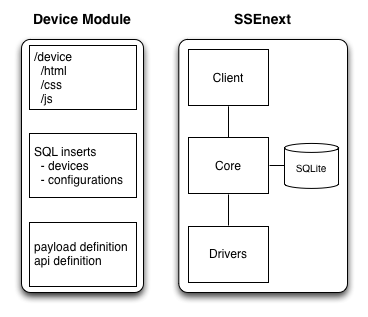
\includegraphics[width=5in]{block_diagram.png} 
\caption{Overview of modular device support.}
\label{fig:blockdiagram}
\end{figure}


This document will explore all three in order.


\section{Client}

TBD - Kumar

\section{Database}

\subsection{Device record}

There needs to be a record in the \verb|records| table for each device
supported by the system.

\subsection{Configuration records}

Depending on the device, SteelSeries may create and include
configurations that are installed as part of the support of that
device. The need to be added to the \verb|configurations| table.



\section{Device interaction}

\subsection{Overview}

The device data flow has three endpoints:
\begin{enumerate}
\item a Lisp file that define the payloads and API calls,
\item the device itself (at least as embodied by the driver layer),
\item json representation of the payloads that goes to/from the application.
\end{enumerate}

This will be discussed in detail below. Figure~\ref{fig:todevice}
shows the data flow of the process of sending settings from the app to a device
while Figure~\ref{fig:fromdevice} shows the flow of data from a device
to the app.

\begin{figure}[htbp] %  figure placement: here, top, bottom, or page
   \centering
   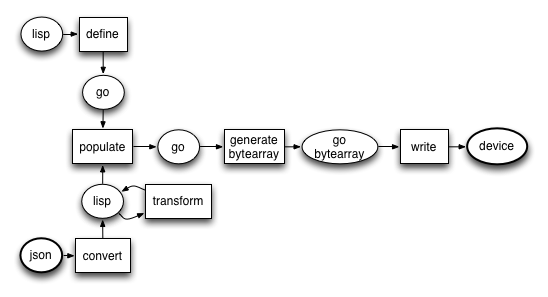
\includegraphics[width=5in]{todevice.png} 
\caption{Overview of modular device support.}
\label{fig:todevice}
\end{figure}

\begin{figure}[htbp] %  figure placement: here, top, bottom, or page
   \centering
   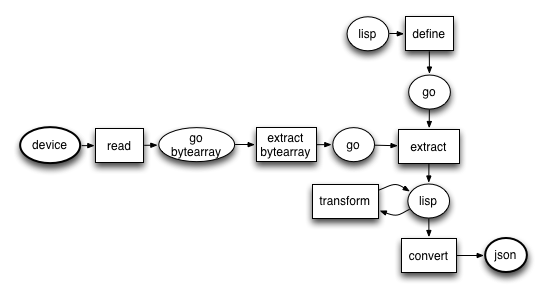
\includegraphics[width=5in]{fromdevice.png} 
\caption{Overview of modular device support.}
\label{fig:fromdevice}
\end{figure}

\subsection{Data definition}
\label{sec:datadefinition}

Each structure defines a conceptually complete chunk of data that
corresponds to what the firmware deals with.  Structures are created
by the \verb|def-struct| function. The first argument to
\verb|def-struct| is the name of the structure as a raw symbol (i.e.
unquoted). \verb|def-struct| can take a number of parameters which
define the fields of the structure.

Each field is defined by \verb|def-field| which takes name and type
(both as raw symbols). The name is an arbitrary symbol (with the
cavaet that it must match the corresponding name in the json used by
\SSEnext. The type must be one of \verb|uint8|, \verb|uint16|,
\verb|uint32|, or the name of another structure. In this example,
that's \verb|led|.

\begin{verbatim}
(def-struct led
     (def-field red uint8)
     (def-field green uint8)
     (def-field blue uint8)
     (def-field mode uint8))

(def-struct cpi
     (def-field unbind uint8)
     (def-field x uint16)
     (def-field y uint16)
     (def-field led led))
\end{verbatim}

These delarations are executed and result in the structure shown in
Figure~\ref{fig:defstructure}. Notice that the individual structures
are separate with inter-structure links being used to denote the
nesting. Note that these structures can be references by any number of
other structures, as well as arrays (more details on this later).

\begin{figure}[htbp] %  figure placement: here, top, bottom, or page
   \centering
   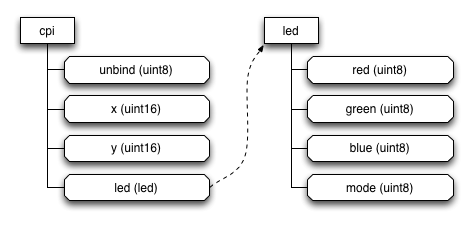
\includegraphics[width=5in]{def_structure.png} 
\caption{Definition structure.}
\label{fig:defstructure}
\end{figure}

That structure then gets processed, flattening it, tagging each field
with it's path in the original structure, and computing the bytearray
offset of each field (to ensure proper alignment). The result is shown
in Figure~\ref{fig:flattened}. Each flattened field also contains the
size of the declared type, and a link to the field node in the
original structure. Note that fields are always ordered by how they
appear in the final bytearray. The order specified in the initial
declaration code carries through to the bytearray.

\begin{figure}[htbp] %  figure placement: here, top, bottom, or page
   \centering
   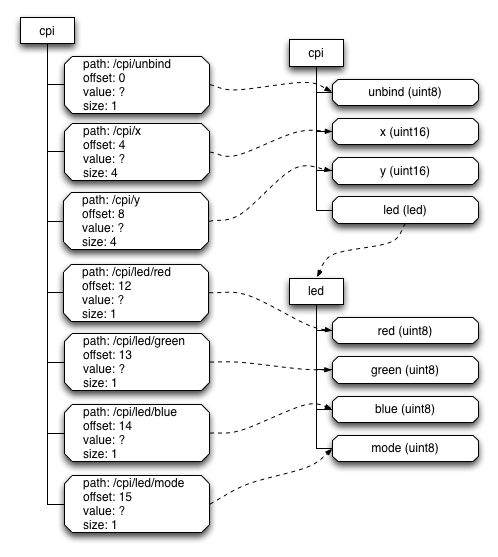
\includegraphics[height=6in]{flat_structure.png} 
\caption{processed structure.}
\label{fig:flattened}
\end{figure}

Notice that each field in the flattened structure contains a value
that is either \verb|uint8|, \verb|uint16|, or \verb|uint32|..
This will initially be 0, and will be filled in later based on either json
from \SSEnext, or bytearray data from the device.

This flattened structure provides a bridge between structured data
containing field values, as json, and the byte array required for
communication with the hardware device. Figure~\ref{fig:bytearray}
shows the bytearray that this structure corresponds to.

\begin{figure}[htbp] %  figure placement: here, top, bottom, or page
   \centering
   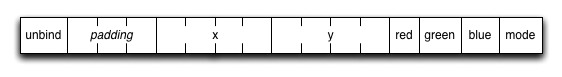
\includegraphics[width=6in]{bytearray.png} 
\caption{The bytearray}
\label{fig:bytearray}
\end{figure}

Fields within a data declaration can be arrayed. When the structure
gets processed/flattened multiple copies of these fields will be
placed in the result. To do this you provide a count using a
\verb|repeat| clause. As an example, here's a declaration that 
contains one simple repeated field and one complex repeated field 
(see the previous structure declaration at the beginning of
\S~\ref{sec:datadefinition}). 

\begin{verbatim}
  (def-struct sensor
     (def-field a uint8 (repeat 4))
     (def-field cpis cpi (repeat 2)))
\end{verbatim}

Once this is processed and flattened, it corresponds to the byte array
shown in Figure~\ref{fig:repeatingbytearray}.

\begin{figure}[htbp] %  figure placement: here, top, bottom, or page
   \centering
   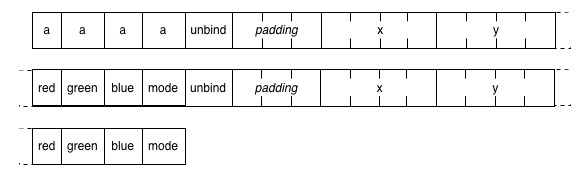
\includegraphics[width=6in]{repeated_bytearray.png} 
\caption{Bytearray with repeating fields}
\label{fig:repeatingbytearray}
\end{figure}

Finally, you can provide a constant value to a field using the
\verb|constant| function:

\begin{verbatim}
   (def-struct current-resolution
     (def-field byte1 uint8
       (constant 0x00))
     (def-field level uint8
       (values 1 2)))
\end{verbatim}

Constant fields have a static value, and are not set from json, and
they are not validated (even if validation criteria are specified).

\subsection{Validation}

All leafs field are a numbers with a valid range given by it's size:
\verb|0x00|-\verb|0xFF| for \verb|uint8|, \verb|0x0000|-\verb|0xFFFF| for \verb|uint16|, and
\verb|0x00000000|-\verb|0xFFFFFFFF| for \verb|uint32|. For some fields the entire range
isn't valid. To enforce this, we introduce validation clauses to the
field definition. There are two types: ranges and values. A range is
specified by lower and upper bounds, which are inclusive. A set of
values is just that: a sequence of valid values for the field. 

\begin{verbatim}
(def-struct cpi
     (def-field unbind uint8
                (values 0 1))
     (def-field x uint16
                (range 0 5670))
     (def-field y uint16
                (range 0 5670))
     (def-field led led))
\end{verbatim}

A \verb|range| validation does no processing on it's arguments; they
are expected to be two non-negative integers in ascending order.

A \verb|values| validation is more flexible in that it can be given a
sequence of numbers that are the valid values, or an
arbitrary expression that will be evaluated with the expectation that
the result is a list of numbers. That list is then used as the set of
valid values for the field.

What was discussed above all happens at the time the structure
declaration is evaluated, and the validation for each field is
completely independant independant all others. Sometimes this isn't
good enough. Conside the following:


\begin{verbatim}
  (def-struct button
    (def-field function uint8
      (values 0 1 2 3 6 8 255))
    (def-field mapping uint8)
    (def-field macro-address uint16
      (range 0 2047))
    (def-field number-of-events uint16
      (range 0 164))
    (def-field debounce-count uint8))
\end{verbatim}

In this example, the \verb|mapping| field's meaning depends on the
value in the \verb|function| field. We need a mechanism to allow us to
compute valid values at validation time as well as inspect the values
in other fields (previous fields will be good enough). And so we have
the \verb|deferred-validation| function:

\begin{verbatim}
  (def-struct button
    (def-field function uint8
      (values 0 1 2 3 6 8 255))
    (def-field mapping uint8
      (deferred-validation (case function
                             (0 (values 1 2 4 8 10))
                             (1 (values 1 255))
                             (2 (range 0 255))
                             (3 (values 0))
                             (6 (values 1 255))
                             (8 (range 0 4))
                             (255 (range 0 255)))))
    (def-field macro-address uint16
      (range 0 2047))
    (def-field number-of-events uint16
      (range 0 164))
    (def-field debounce-count uint8))
\end{verbatim}

In the above example, the validation for \verb|mapping| specifies some
code to be run when the field is to be validated. In this case it's a
\verb|case| that branches based on the value in the \verb|function| field,
choosing the appropriate \verb|range| or \verb|values|.

\subsection{Directional declarations}

So far we've seen how to create a simple structure that will be used
for communication with the device api: using the same structure for
writing to and reading from the api. If the structre used for data returned from a
specific api command differs from that used when sending the command,
you can define separate \verb|outgoing| and \verb|incoming| structures:

\begin{verbatim}
  (def-struct resolution
    (outgoing
      (def-field level uint8
        (values 1 2))
      (def-field cpi uint8))
    (incoming
      (def-field cpi uint8)))
\end{verbatim}

In the above declaration the \verb|outgoing| structure consists of a
level specifier and a cpi value, while the \verb|incoming| structure
contains only a cpi field.

Any communication being sent to the device will use the
\verb|outgoing| structure, and any data returned by the device will
be extracted using the \verb|incoming| structure.

If you just need to declare a single
structure, you {\bf can} use a \verb|common| clause, as so:

\begin{verbatim}
  (def-struct cpi
    (common
      (def-field unbind uint8 (values 0 1))
      (def-field x uint16 (range 0 5670))
      (def-field y uint16 (range 0 5670))
      (def-field led led)))
\end{verbatim}

Alternatively, you can just declare the bare fields, as so:

\begin{verbatim}
  (def-struct cpi
    (def-field unbind uint8 (values 0 1))
    (def-field x uint16 (range 0 5670))
    (def-field y uint16 (range 0 5670))
    (def-field led led))
\end{verbatim}

\subsection{Json}

Now that we've covered the data interaction with the device firmware,
let us turn to the communication to the \SSEnext application. \SSEnext
deals in json, specifically json that is parallel to the structure we've
declared. Going back to the structure declaration at the beginning of
\S~\ref{sec:datadefinition}, we will want json of the form:

\begin{verbatim}
{
  "cpi": {
    "unbind": 1,
    "x": 1200,
    "y": 1400,
    "led": {
      "red": 255,
      "green": 255,
      "blue": 100,
      "mode": 2
    }
  }
}
\end{verbatim}

When this jason is received by the device support layer, it gets
processed and converted to a Lisp structure: 

\begin{verbatim}
(("cpi" . (("unbind" . 1)
           ("x" . 1200)
           ("y" . 1400)
           ("led" . (("red" . 255)
                     ("green" . 255)
                     ("blue" . 100)
                     ("mode". 2))))))
\end{verbatim}

Numbers stay numbers (integers to be specific), key strings stay
strings, arrays become lists (e.g. \verb|[1, 2, 3]| $\Rightarrow$
\verb|(1 2 3)|, and maps being association lists (e.g.
\verb|{"a": 3, "b": 4}| $\Rightarrow$ \verb|(("a" . 3)("b" . 4))|).

When using json to populate the values in the fields, the paths from
the fields are used to traverse the json to find the corresponding
values. Once values are in the fields, they are validated, and the
flattened structure can be used to generate the bytearray.

Conversely, the data in a bytearray can be extracted based on the
offsets and sizes in the fields and used to set the values in those
fields. Once the field values are populated, the corresponding paths
can be used to build an appropriate json structure that can be sent to
\SSEnext. 

\subsection{JSON transformations}

In the last section we went over how to declare fields, providing a
name, type, and possibly a repeat count and validation. You can
optionally provide two more clauses that will effect the consumption and
generation of json related to the field.

These two additional clauses are Lisp functions (either named or
anonymous lambdas) that are used to transform the json as it is on
it's way to the app, or on its way from the app. These functions take
two arguments:

\begin{enumerate} 
\item the value from the json node corresponding
to the field, and
\item the json node containing it. 
\end{enumerate}

The functions return nothing but can modify or replace the
corresponding value in the json structure.

As an example here's how to handle the name field on a Sensei. In the
structure it is an array of 16 \verb|uint8|s, while in json it should
be a string. This assumes functions \verb|(bytes-to-string bytes)| and
\verb|(string-to-bytes string)|

\begin{verbatim} 
(def-struct profile
     (def-field id uint8)
     (def-field name uint8 
                (repeat 16)
                (to-json (lambda (bytes parent)
                           (acons "name" (bytes-to-string bytes) parent)))
                (from-json (lambda (str parent)
                             (acons "name" (string-to-bytes str) parent))))
     (def-field size uint16)
     ...)
\end{verbatim}

\noindent For this declaraion, given that the json derived from the
bytearray read from the device looks like:

\begin{verbatim}
  ("profile" . (("id" . 3)
                ("name" . (48 49 50 51 52 53 54 55 56 57 
                           00 00 00 00 00 00))
                ...))
\end{verbatim}

\noindent it would be transformed to the following before being sent
to the app:

\begin{verbatim}
  ("profile" . (("id" . 3)
                ("name" . "0123456789")
                ...))
 
\end{verbatim}

\noindent The other transform would change the json in the opposite
direcion, right padding the bytearray with \verb|0|s to make the
required 16 bytes.

\subsection{API definition}

\begin{verbatim}
  (def-api profile
    [<sexpr>...]
    (read <protocol> (chunk <type> <size> <sexpr>)...)
    [<sexpr>...]
    (write <protocol> (chunk <type> <size> <sexpr>)...))
\end{verbatim}

\noindent An API endpoint can be defined for any structure that needs
to be read and/or written to the device. The core of an API
declaration are the read and write clauses (both of which are
optional). The structure is the same in each case: a protocol specifier
(a \verb|uint32|) followed by a sequence of chunk declarations. A chunk
declaration is made up of type value (a \verb|uint32|), the size of the chunk's
data (a \verb|uint32|), and an sexpr that evaluates to a bytearray which can be
no longer than the size specified. Note that the generated bytearray
can be shorter than the stated size: the allocated byte array will be
padded with zeros.

For convienence, there are predefined protocol specifiers:

\begin{itemize}
\item \verb|HID|
\item \verb|X2|
\item \verb|KNX|
\item \verb|SSE|
\end{itemize}

When the chunks are being serialized into a byte array (using the
sexprs) the \verb|payload| symbol is available that evaluates to the
serialized payload byte array as defined by the corresponding
structure using the provided json data. There is also a handy function
for changing bytes in a bytearray:

\begin{verbatim}
  (replace-byte <bytearray> <position> <new value>)
\end{verbatim}

The position is zero-based and the new value must be a byte value
(0-255). The byte array has to be an object reprtesenting a bytearray.
E.g. the result of evaluating \verb|payload|.

There is also a way to extract a byte from a bytearray:

\begin{verbatim}
  (extract-byte <bytearray> <position>)
\end{verbatim}

Sopmetimes you will need a literal bytearray, either foir a literal
payload, or an a template on which you'll use \verb|replace-byte|.

\begin{verbatim}
  (list-to-bytearray <list of bytes>)

  (list-to-bytearray '(1 2 3 4 5))
\end{verbatim}

There are times (e.g. an initialization sequence) when tyou will need
to do a low level, raw wrtiter to a device. You can use the function
\verb|raw-write-to-device| to accomplish this.

\begin{verbatim}
  (raw-write-to-device <byte array>)

  (raw-write-to-device (list-to-bytearray '(1 2 3 4 5))
\end{verbatim}

Some devices need some initialization, such as a specific init/config
command. This can be done by using \verb|def-init| to attach init code
to the device.

\begin{verbatim}
  (def-init <sexpr>...)
\end{verbatim}

There is the capability to have arbitrary sexprs before and/or after
the read/write decalrations. Beyond that, the read/write declarations
can be embedded in a let, etc. They know the API declaration in which
they are being evaluated, so they do not have to be in the API
declarations immediate context.

Json coming from core has a top level key that matches the name of
both a structure and an api. The data indexed by that key is used to
build the payload bytearray from the structure with the same name,
which is then available to the API read/write commands.



\subsection{Example: an illustrative test case}

This is extracted from a test case of the API layer.  We start with a device declaration:

\begin{verbatim}
(def-device sensei-raw 
  (def-struct test 
    (outgoing (def-field f uint8 (repeat 4)))
    (incoming (def-field g uint8)))
  (def-api test
    (read HID (chunk 0 4 payload))))
\end{verbatim}

This test device has one endpoint defined by one structure and one
api. The structure has an outgoing format with field \verb|f| that is
an array of 4 bytes, and an incoming structure of a field \verb|g|
that is a single byte. The api declares a single chunk containing a 4
byte payload.

We'll use the following json to define the payload data:

\begin{verbatim}
{
  "test": {
    "f": [1, 2, 3, 4]
  }
}
\end{verbatim}

This specifies the structure and api \verb|test| and the value of the
field \verb|f|. In the test, we specify that the read should return
the byte \verb|255|, we get back the json:

\begin{verbatim}
{
  "test":{
    "g":255
  }
}
\end{verbatim}

\subsection{Example: sensei-raw.device}

As an example, here's the full declaration of the Sensei[RAW] device:

\begin{verbatim}
(def-device sensei-raw

  (def-struct resolution
    (outgoing
     (def-field level uint8
       ;; which level (of two) is this pertains to
       (values 1 2))
     (def-field cpi uint8
       ;; N, where the resolution is N * 90
       ))
    (incoming
     (def-field cpi uint8
       ;; N, where the resolution is N * 90
       )))
    
  (def-struct polling-rate
    (outgoing
     (def-field cmd uint8
       (constant 0x00))
     (def-field byte1 uint8
       (constant 0x00))
     (def-field rate uint8
       (values
        1                                ; 1000 Hz
        2                                ; 500 Hz
        3                                ; 250 Hz
        4                                ; 125Hz
        )))
    (incoming
     (def-field rate uint8
       (values
        1                                ; 1000 Hz
        2                                ; 500 Hz
        3                                ; 250 Hz
        4                                ; 125 Hz
        ))))                     
  
  (def-struct led-brightness
    (outgoing
     (def-field cmd uint8
       (constant 0x00))
     (def-field index uint8
       (constant 0x01))
     (def-field brightness uint8
       (values
        1                                ; off
        2                                ; low brightness
        3                                ; medium brightness
        4                                ; high brightness
        )))
    (incoming
     (def-field brightness uint8
       (values
        1                                ; off
        2                                ; low brightness
        3                                ; medium brightness
        4                                ; high brightness
        ))))

  (def-struct current-resolution
    (outgoing
     (def-field cmd uint8
       (constant 0x00))
     (def-field byte1 uint8
       (constant 0x00))
     (def-field level uint8
       (values 1 2)))
    (incoming
     (def-field level uint8
       (values 1 2))))

  (def-struct led-pulsation
    (outgoing
     (def-field cmd uint8
       (constant 0x00))
     (def-field index uint8
       (constant 0x01))
     (def-field speed uint8
       (values
        1                                ; steady
        2                                ; pulsation slow
        3                                ; pulsation medium
        4                                ; pulsatioon fast
        5)))
    (incoming
     (def-field speed uint8
       (values
        1                                ; steady
        2                                ; pulsation slow
        3                                ; pulsation medium
        4                                ; pulsatioon fast
        5))))                             ; trigger mode

  (def-struct save-profile-settings
    (def-field cmd uint8
      (constant 0x09))
    (def-field byte1 uint8
      (constant 0x00)))

  (def-api resolution
    (read HID (chunk 0 32 (replace-byte payload 0 0x13)))
    (write HID (chunk 0 32 (replace-byte payload 0 0x03))))

  (def-api polling-rate
    (read HID (chunk 0 32 (replace-byte payload 0 0x14)))
    (write HID (chunk 0 32 (replace-byte payload 0 0x04))))

  (def-api led-brightness
    (read HID (chunk 0 32 (replace-byte payload 0 0x15)))
    (write HID (chunk 0 32 (replace-byte payload 0 0x05))))

  (def-api current-resolution
    (read HID (chunk 0 32 (replace-byte payload 0 0x16)))
    (write HID (chunk 0 32 (replace-byte payload 0 0x06))))

  (def-api led-pulsation
    (read HID (chunk 0 32 (replace-byte payload 0 0x17)))
    (write HID (chunk 0 32 (replace-byte payload 0 0x07))))

  (def-api save-profile-settings
    (write HID (chunk 0 32 payload))))
\end{verbatim}

\end{document}
